\documentclass[11pt,a4paper]{article}

\usepackage{graphicx}
\usepackage{xcolor}
\usepackage{geometry}
\geometry{a4paper, top=2.5cm, bottom=2.5cm, left=2.5cm, right=2.5cm}
\usepackage{amsmath}
\usepackage{booktabs}
\usepackage{tabularx}
\newcolumntype{Y}{>{\raggedright\arraybackslash}X}
\usepackage{adjustbox}
\usepackage{enumitem}
\usepackage{microtype}
\usepackage{placeins}
\usepackage{tikz}
\usetikzlibrary{arrows.meta,positioning}
\usepackage[numbers,sort&compress]{natbib}
\bibliographystyle{unsrtnat}
\usepackage[colorlinks=true, linkcolor=blue, citecolor=blue!60!black, urlcolor=blue, bookmarks=true, bookmarksnumbered=true, unicode=true]{hyperref}

\hypersetup{
    pdftitle={MindfulAI: A Privacy-First Multi-Modal Framework for Emotion-Aware Mental Wellness Support},
    pdfauthor={Aditya Yadav},
    pdfsubject={Affective computing, mental health informatics, privacy by design},
    pdfkeywords={mental wellness, emotion classification, privacy by design, conversational agents, multi-modal affective computing}
}

\widowpenalty=10000
\clubpenalty=10000

\renewcommand{\topfraction}{0.92}
\renewcommand{\bottomfraction}{0.6}
\renewcommand{\floatpagefraction}{0.85}

\newcommand{\system}{MindfulAI}

\begin{document}

\begin{center}
    {\LARGE\bfseries \system{}: A Privacy-First Multi-Modal Framework\\[2pt] for Emotion-Aware Mental Wellness Support\par}
    \vspace{10pt}
    {\large Aditya Yadav\par}
    \vspace{4pt}
    {\normalsize Department of Computer Science \& Engineering, Kolkata, India\par}
    {\normalsize \texttt{github.com/adineo-cmd/mindfulai}\par}
    \vspace{6pt}
    {\normalsize November 2026\par}
\end{center}

\vspace{8pt}

\begin{abstract}
\noindent Conversational agents and smartphone applications for mental wellness have shown encouraging but uneven results: meta-analytic evidence supports small but reliable symptom reductions, while objective usage analyses reveal steep real-world engagement decay and widespread privacy deficiencies in deployed applications. This paper presents \system{}, a privacy-first, multi-modal mental wellness platform that unifies three complementary affective signals---written journal text, live facial video, and explicit daily self-report---into a single derived-label store. Text is analyzed with a DistilRoBERTa transformer over a seven-class emotion taxonomy, facial expression is classified by a Vision Transformer operating on a consent-gated WebSocket stream at approximately one inference per second, and self-reported mood provides an explicit ground truth for longitudinal correlation analysis. Critically, the system never persists raw video or audio: only derived emotion labels reach the database, and users are provided with full data portability and hard-deletion rights consistent with GDPR Article 17. We position \system{} against the best-documented prior systems---the conversational agents Woebot, Wysa, and Tess---and show through a structured comparison that its distinguishing contributions lie in modality breadth, emotion granularity, retention policy, transparency of crisis handling, and reproducibility, rather than in unproven clinical efficacy claims. We additionally propose a preregistered two-armed pilot protocol capable of testing the design against published benchmarks, and we discuss limitations, including the contested validity of facial expression inference and the risks of LLM-generated supportive dialogue.
\end{abstract}

\vspace{4pt}
\noindent\textbf{Keywords:} affective computing; mental health informatics; conversational agents; privacy by design; emotion classification; digital phenotyping

\vspace{6pt}

\section{Introduction}\label{sec:intro}

Common mental health problems such as depression and anxiety remain substantially under-treated worldwide, and app-supported smartphone interventions have emerged as a scalable complement to formal care. A meta-analysis of randomized controlled trials found that smartphone interventions outperform control conditions for depressive symptoms ($g = 0.28$, 54 trials) and generalized anxiety symptoms ($g = 0.30$, 39 trials)~\cite{linardon2019}. Yet two structural weaknesses constrain this literature and the products built upon it.

The first weakness is \emph{engagement}. An objective, panel-based analysis of popular mental health applications found that real-world usage is low and decays sharply within the first month of installation~\cite{baumel2019}. Applications that rely on a single interaction channel---typically typed conversation with a chatbot or manual questionnaire entry---offer few reasons for a user to return, and self-report fatigue accumulates quickly.

The second weakness is \emph{privacy}. Independent evaluations of consumer mental health applications repeatedly document missing or weak privacy policies and unspecified data-sharing practices, even though the data involved is among the most sensitive a person can disclose~\cite{lagan2020}. Reviews of chatbots for mental health catalog a wide range of agent designs but note that safety assessment is rare in the underlying studies~\cite{abdalrazaq2019,abdalrazaq2020}.

This paper introduces \system{}, an open, self-hostable mental wellness platform designed against both weaknesses simultaneously. \system{} reduces the reliance on any single channel by fusing three complementary signals of affective state: what the user \emph{writes} (journal entries analyzed by a transformer), what the user's \emph{face shows} (a consent-gated live video stream classified by a Vision Transformer), and what the user \emph{says about themselves} (daily emoji and slider check-ins). All three channels are reduced to derived emotion labels before storage; raw video and audio are never persisted. The platform couples this pipeline with per-user consent records, complete JSON data export, GDPR-consistent hard deletion, and a crisis-detection path that escalates to human-support resources rather than continuing a bot conversation.

The contributions of this paper are fourfold:
\begin{enumerate}[leftmargin=2em, itemsep=2pt]
    \item \textbf{A unified multi-modal derived-label architecture} in which journal text, live facial video, and explicit self-report are normalized to a single longitudinal label store, with a hard architectural guarantee that raw media are never persisted.
    \item \textbf{Fine-grained emotion representation.} Instead of binary sentiment, text is mapped to a seven-class emotion taxonomy (anger, disgust, fear, joy, neutral, sadness, surprise) consistent with modern fine-grained emotion datasets~\cite{demszky2020,hartmann2023}, and self-reported mood is retained separately so that inferred and felt emotion can be compared over time.
    \item \textbf{Privacy by design as an architectural property rather than a policy statement}: consent gating for the camera path, derivation-before-storage, JSON portability, and GDPR Article 17 hard deletion~\cite{gdpr2016}.
    \item \textbf{A transparent comparison and a validation path.} We provide a structured comparison against Woebot~\cite{fitzpatrick2017}, Wysa~\cite{inkster2018}, and Tess~\cite{fulmer2018}---the best-documented agents in the literature---and specify a preregistered pilot protocol that would allow the design to be evaluated against published benchmarks.
\end{enumerate}

We deliberately refrain from claiming clinical effectiveness: no randomized trial of \system{} has been conducted, and Section~\ref{sec:eval} specifies exactly what evidence is still missing and how to obtain it. The aim of this paper is to demonstrate that the \emph{design space} of wellness applications includes positions that prior widely-deployed systems do not occupy, and to make those positions explicit, reproducible, and testable.

\section{Related Work}\label{sec:related}

\subsection{Conversational Agents for Mental Health}\label{sec:agents}

Automated supportive dialogue began with Weizenbaum's ELIZA~\cite{weizenbaum1966}, and the modern generation of mental health chatbots inherits both its promise and its cautions. Abd-Alrazaq et al.\ provide the most complete feature-level overview, describing chatbots that deliver psychoeducation, screening, and therapeutic exercises, and observing that user-facing features vary widely while safety evaluation is uncommon~\cite{abdalrazaq2019}. Their subsequent meta-analysis found weak but directionally positive evidence that chatbots improve depression, distress, and stress outcomes, with only two studies assessing safety~\cite{abdalrazaq2020}.

Three agents anchor the empirical literature. Woebot was evaluated in a two-arm randomized controlled trial with young adults reporting symptoms of depression and anxiety: over two weeks, participants interacted with the fully automated CBT agent an average of 12.14 times and showed significantly greater PHQ-9 reductions than an information-only control~\cite{fitzpatrick2017}. Wysa, an empathy-oriented self-help agent, was evaluated with a mixed-methods real-world dataset linking in-app engagement to depressive symptom trajectories~\cite{inkster2018}. Tess, a relational agent delivered over SMS and voice, reduced symptoms of depression and anxiety in a randomized trial relative to psychoeducation~\cite{fulmer2018}. All three are text-centric. Large language models have since raised the ceiling of dialogue quality: in a cross-sectional comparison of responses to real patient questions, evaluators preferred chatbot responses to physician responses in 78.6\% of cases and rated them higher on both quality and empathy~\cite{ayers2023}---a finding that motivates \system{}'s LLM-based companion module, while also sharpening the safety obligations that Section~\ref{sec:limitations} discusses.

\subsection{App Efficacy and Engagement}\label{sec:efficacy}

Beyond chatbots, meta-analytic evidence places app-supported interventions as modest but reliable adjuncts to care~\cite{linardon2019}. The engagement problem, however, is persistent: objective usage telemetry shows that most users of mental health applications abandon them within weeks~\cite{baumel2019}. Two design responses recur in the literature: reducing the friction of each interaction, and diversifying the channels through which a user can contribute meaningful data. Written emotional disclosure, the act underlying journaling, additionally carries a long-studied therapeutic tradition in its own right~\cite{pennebaker1997}. \system{} takes the diversification response further than prior systems by supporting typed reflection, passive-with-consent facial analysis, and lightweight self-report in one coherent data model.

\subsection{Affective Computing and Multi-Modal Fusion}\label{sec:affective}

Affective computing has progressed from unimodal analysis (text, audio, facial expression, physiological signals) toward multi-modal fusion, with fusion strategies ranging from early feature-level combination to late decision-level aggregation~\cite{poria2017}. In the text channel, large pretrained transformers have made fine-grained emotion classification practical: GoEmotions established a 27-category human-annotated benchmark~\cite{demszky2020}, and Hartmann et al.\ benchmarked publicly available sentiment and emotion models---including the seven-class DistilRoBERTa classifier used in this work---showing that model choice materially changes downstream conclusions~\cite{hartmann2023}. Transformer architectures also underpin modern facial expression analysis; the Vision Transformer~\cite{dosovitskiy2021} is the classification backbone for \system{}'s live facial channel, and distillation techniques~\cite{sanh2019,liu2019} make the text-side model deployable on commodity hardware.

An important counter-current grounds our treatment of the facial channel: Barrett et al.\ demonstrate that inferring a person's \emph{felt} emotion from facial movements is far less reliable than commonly assumed~\cite{barrett2019}. \system{} therefore treats facial labels as one approximate, consent-gated signal among three, never as ground truth, and retains the user's explicit self-report as the reference signal for longitudinal comparison.

\subsection{Privacy and App Evaluation}\label{sec:privacy}

Lagan et al.\ translated expert evaluation frameworks into objective metrics across privacy, security, evidence, and accessibility, and found pervasive deficits in marketplace applications~\cite{lagan2020}. \system{}'s contribution here is architectural: privacy-relevant behavior is enforced by the data pipeline (derivation before storage; per-user consent records; deletion as a hard, complete operation) rather than delegated to a policy document. Data protection regulation grants individuals the right to erasure~\cite{gdpr2016}; \system{} implements that right as a single destructive API operation backed by cascading database deletes.

\section{System Architecture}\label{sec:arch}

\subsection{Overview}

\system{} is a two-tier web application. The front end is a static-first Astro site with React islands for interactive panels (dashboard, journal, live facial check, trends, settings). The back end is a FastAPI service exposing a REST API and two WebSocket streams, backed by SQLAlchemy 2.0 over SQLite in development and PostgreSQL in production. Figure~\ref{fig:arch} shows the signal flow: all three input channels converge on a single derived-label store that feeds analytics, trend visualizations, and data export.

\begin{figure}[t]
\centering
\resizebox{0.94\columnwidth}{!}{%
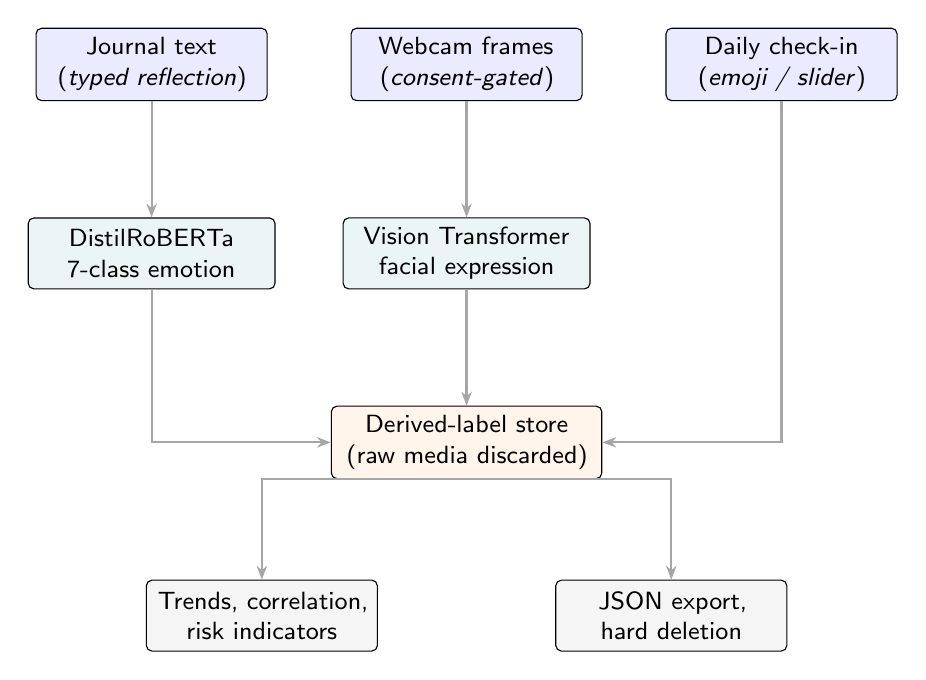
\begin{tikzpicture}[
  input/.style={draw, rounded corners=2pt, text width=2.7cm, minimum height=0.9cm, align=center, font=\small\sffamily, fill=blue!8},
  model/.style={draw, rounded corners=2pt, text width=2.9cm, minimum height=0.9cm, align=center, font=\small\sffamily, fill=teal!8},
  store/.style={draw, rounded corners=2pt, text width=3.2cm, minimum height=0.9cm, align=center, font=\small\sffamily, fill=orange!8},
  output/.style={draw, rounded corners=2pt, text width=2.7cm, minimum height=0.9cm, align=center, font=\small\sffamily, fill=gray!8},
  arr/.style={-{Stealth[length=5pt]}, thick, gray!70}
]
  \node[input] (journal) at (0,0) {Journal text\\(\emph{typed reflection})};
  \node[input] (camera) at (4.0,0) {Webcam frames\\(\emph{consent-gated})};
  \node[input] (checkin) at (8.0,0) {Daily check-in\\(\emph{emoji / slider})};
  \node[model] (textmodel) at (0,-2.4) {DistilRoBERTa\\7-class emotion};
  \node[model] (vitmodel) at (4.0,-2.4) {Vision Transformer\\facial expression};
  \node[store] (store) at (4.0,-4.8) {Derived-label store\\(raw media discarded)};
  \node[output] (analytics) at (1.4,-7.0) {Trends, correlation,\\risk indicators};
  \node[output] (export) at (6.6,-7.0) {JSON export,\\hard deletion};
  \draw[arr] (journal.south) -- (textmodel.north);
  \draw[arr] (camera.south) -- (vitmodel.north);
  \draw[arr] (checkin.south) |- (store.east);
  \draw[arr] (textmodel.south) |- (store.west);
  \draw[arr] (vitmodel.south) -- (store.north);
  \draw[arr] (store.south) -| (analytics.north);
  \draw[arr] (store.south) -| (export.north);
\end{tikzpicture}
}
\caption{\system{} signal flow. Three input channels are reduced to derived emotion labels before persistence; raw video is processed in memory and discarded. Explicit self-report is retained as the user's own ground truth alongside inferred labels.}
\label{fig:arch}
\end{figure}

\subsection{Multi-Modal Emotion Pipeline}\label{sec:pipeline}

Table~\ref{tab:modalities} summarizes the three channels. Each channel produces timestamped, user-scoped records of a common shape (emotion label, confidence, modality-specific metadata), which the analytics layer aggregates independently of source.

\begin{table}[t]
\centering
\small
\caption{The three affective channels and their persistence behavior.}
\label{tab:modalities}
\begin{tabularx}{\columnwidth}{@{}l Y Y Y@{}}
\toprule
 & \textbf{Journal text} & \textbf{Live facial check} & \textbf{Self-report} \\
\midrule
Model & DistilRoBERTa, 7-class emotion classifier~\cite{hartmann2023,sanh2019} & ViT facial expression classifier~\cite{dosovitskiy2021}; Haar-cascade pre-crop~\cite{violajones2001} & User-entered emoji and slider value \\
Granularity & Seven classes: anger, disgust, fear, joy, neutral, sadness, surprise & Discrete expression labels per frame & Continuous subjective mood \\
Transport & REST on journal save & WebSocket stream, throttled to $\approx$1 inference/s & REST on check-in \\
Persisted & Label + confidence + timestamp & Label + timestamp only; \textbf{frames never stored} & Raw user value \\
Fallback & VADER lexicon polarity~\cite{hutto2014} & Session stops on consent withdrawal & None \\
\bottomrule
\end{tabularx}
\end{table}

Text entries are classified by the seven-class DistilRoBERTa emotion model, whose taxonomy descends from the fine-grained emotion tradition of GoEmotions~\cite{demszky2020} and whose relative accuracy profile is characterized in the Hartmann et al.\ benchmark~\cite{hartmann2023}. A VADER polarity score is computed as a near-instant fallback signal when the transformer is unavailable~\cite{hutto2014}. The seven-class choice follows the emotion-theoretic tradition of discrete basic emotions~\cite{ekman1992} while remaining fine-grained enough to distinguish, for example, sadness from fear in longitudinal trends.

The live facial channel is explicitly opt-in. A per-user consent record gates the entire path: with consent off, no camera capture occurs at any layer, and unchecking consent immediately terminates the WebSocket session. When active, frames are streamed over WebSocket, pre-cropped by a Haar cascade detector~\cite{violajones2001}, and classified by a ViT-based expression model~\cite{dosovitskiy2021} at approximately one inference per second to bound CPU load. Frames exist only in memory for the duration of a classification; the only artifacts written to the database are the resulting label and timestamp. Self-reported mood is captured through a daily check-in and serves as the explicit reference signal for the correlation analyses described next.

The analytics layer computes mood trend lines, emotion distributions, weekly heatmaps, stress and burnout risk indicators, and---uniquely enabled by the multi-modal design---a longitudinal \emph{correlation between inferred facial emotion and explicit self-report}, which operationalizes the discrepancy between displayed and felt affect~\cite{barrett2019,poria2017} as an inspectable per-user metric.

\subsection{Supportive Dialogue and Crisis Escalation}\label{sec:chat}

A companion chat module provides supportive conversation through a locally hosted LLM, degrading gracefully to a deterministic mock response when no model endpoint is configured. Every user message is scanned by a crisis-keyword detector before generation; when triggered, the pipeline bypasses the language model entirely and returns a structured \texttt{requires\_\allowbreak human\_\allowbreak support} response that surfaces crisis resources. This is a deliberate inversion of the usual chatbot-first design: automated dialogue is treated as acceptable only in the space where human escalation has not been indicated. The design is informed both by the demonstrated quality of LLM supportive responses~\cite{ayers2023} and by the safety gaps documented for deployed mental health chatbots~\cite{abdalrazaq2019,abdalrazaq2020}.

\subsection{Identity Binding}

An auxiliary module supports optional face enrollment: a user may upload a reference photo, from which a Facenet embedding is computed and stored so that a live facial session can be bound to the correct account via cosine similarity (threshold $0.85$). Reference images are stored outside version control by configuration, precisely because enrolling biometric material into a repository or a shared artifact pipeline would create a disclosure hazard; embeddings, not images, are the only derived identity data retained.

\subsection{Privacy Operations}

Two operations complete the privacy posture. First, \texttt{GET /api/user/data} returns a complete JSON export of every record linked to the requesting account, satisfying data portability. Second, \texttt{DELETE /api/user/data} performs a hard, cascading deletion of all user-scoped records---mood logs, text and facial emotion records, consent records, and account material---implementing erasure as an executable guarantee consistent with GDPR Article 17~\cite{gdpr2016}. Aggregate analytics are computed server-side and never expose individual records across accounts.

\section{Comparison with Prior Systems}\label{sec:comparison}

\begin{table}[t]
\centering
\small
\caption{\system{} versus the best-documented prior conversational agents for mental wellness. Entries for prior systems are restricted to what their cited evaluations state; ``not reported'' indicates the dimension is not disclosed in the cited source.}
\label{tab:comparison}
\begin{tabularx}{\columnwidth}{@{}>{\raggedright\arraybackslash}p{2.35cm} Y Y Y Y@{}}
\toprule
\textbf{Dimension} & \textbf{\system{}} & \textbf{Woebot~\cite{fitzpatrick2017}} & \textbf{Wysa~\cite{inkster2018}} & \textbf{Tess~\cite{fulmer2018}} \\
\midrule
Interaction modality & Journal text + live facial video + daily self-report & Structured CBT dialogue (text) & Text-based empathetic self-help dialogue & SMS text and voice messages \\
\addlinespace
Emotion representation & 7-class transformer taxonomy + VADER fallback + raw self-report & Outcome scales (PHQ-9, GAD-7); in-app taxonomy not reported & In-app emotion model not reported & Symptom scales as outcomes; in-app taxonomy not reported \\
\addlinespace
Raw media retention & None; derived labels only & No camera channel & No camera channel & No camera channel \\
\addlinespace
Consent mechanism & Per-user consent record gating all camera activity; immediate session termination on withdrawal & Not reported & Not reported & Not reported \\
\addlinespace
Crisis handling & Keyword detector bypasses LLM and returns \texttt{requires\_\allowbreak human\_\allowbreak support} with resources & Not reported in cited trial & Not reported in cited study & Not reported in cited trial \\
\addlinespace
Portability \& erasure & Full JSON export; hard cascading deletion (GDPR Art.~17)~\cite{gdpr2016} & Not reported & Not reported & Not reported \\
\addlinespace
Model openness & Open pretrained transformers; self-hostable stack & Proprietary & Proprietary & Proprietary \\
\addlinespace
Evidence base & System-level validation; preregistered trial protocol proposed (\S\ref{sec:eval}) & Two-arm RCT, 2 weeks, PHQ-9 improvement & Mixed-methods real-world study & Randomized trial \\
\bottomrule
\end{tabularx}
\end{table}

Table~\ref{tab:comparison} compares \system{} against Woebot, Wysa, and Tess along eight dimensions, using only what the cited evaluations report. Empty capability claims are marked ``not reported'' rather than inferred.

Three observations follow from Table~\ref{tab:comparison}.

\textbf{Modality breadth is genuinely novel at this evidence tier.} Woebot, Wysa, and Tess each proved that a single, well-executed text channel can produce measurable benefit~\cite{fitzpatrick2017,inkster2018,fulmer2018}. \system{} is positioned differently: by normalizing three channels into one derived-label store, it captures affect at different latencies (instantaneous facial labels, reflective journal labels, deliberate self-report) and makes their disagreement itself an analytical object~\cite{poria2017}.

\textbf{Privacy-relevant behavior is architectural, not documentary.} The evaluations of prior agents do not report retention policy for conversational data, consent workflows, or erasure mechanisms, while independent app evaluations document pervasive privacy deficits across the marketplace~\cite{lagan2020}. \system{} makes retention policy falsifiable: one can verify from the schema that no table stores raw media, and from the API that deletion is total.

\textbf{Transparency extends to the evidence boundary.} \system{} currently offers system-level validation only; where prior systems have RCT evidence, the table says so. The design claim is therefore modest and checkable: \system{} occupies a region of the design space---multi-modal, retention-free, consent-gated, self-hostable, escalation-transparent---that the trial-proven agents, as reported, do not.

\FloatBarrier

\section{Design Rationale}\label{sec:rationale}

Five principles generate the architecture of Section~\ref{sec:arch}, each traceable to a documented failure mode of prior systems.

\begin{enumerate}[leftmargin=2em, itemsep=3pt]
    \item \textbf{Derive before persist.} Raw video and audio are the highest-liability assets a wellness platform can hold~\cite{lagan2020}; \system{}'s pipeline classifies in memory and persists labels only, removing the asset class entirely rather than protecting it.
    \item \textbf{Consent gates the sensor, not a checkbox.} The consent record is consulted by every layer of the camera path, and withdrawal acts immediately---closing the gap between a settings page and actual data flow.
    \item \textbf{Granular emotions over binary sentiment.} Seven-class classification preserves distinctions (sadness vs.\ fear, joy vs.\ surprise) that binary polarity erases~\cite{demszky2020,hartmann2023}, and those distinctions are what make longitudinal emotion trajectories interpretable.
    \item \textbf{Inferred labels are never treated as truth.} Consistent with the facial-expression validity critique~\cite{barrett2019}, the facial channel is one approximate signal among three, and the explicit self-report anchors the analytics; the platform even visualizes their divergence rather than hiding it.
    \item \textbf{Escalate to humans at the boundary.} Crisis detection short-circuits automated dialogue~\cite{abdalrazaq2020}, and supportive LLM dialogue is positioned as an adjunct whose quality benchmark~\cite{ayers2023} never removes the obligation to escalate.
\end{enumerate}

\section{Evaluation and Proposed Validation}\label{sec:eval}

\subsection{Current System-Level Validation}

\system{} is validated today at the engineering level, and we report this scope honestly. The service layer carries an automated test suite covering text classification, facial-emotion processing, and analytics aggregation. The facial pipeline is throttled to approximately one inference per second, bounding worst-case CPU load per concurrent session. Degradation paths are exercised by design: without an LLM endpoint the chat module returns mock responses; without the transformer service available, journal classification falls back to VADER~\cite{hutto2014}; without consent, no camera component activates. Data-privacy invariants are structural: the persistence schema contains no raw-media columns, and the erasure endpoint deletes every user-scoped record.

\subsection{A Preregistered Pilot Protocol}

The missing evidence is clinical and behavioral. We propose the following preregistered, two-armed, eight-week pilot, designed so that results are directly comparable with the published benchmarks cited in this paper:

\begin{itemize}[leftmargin=2em, itemsep=2pt]
    \item \textbf{Population:} adults with elevated depressive or anxiety symptoms (PHQ-9 or GAD-7 above threshold), excluding acute crisis presentations, who consent to all three channels.
    \item \textbf{Arms:} \system{} ($n \approx 60$) versus an attention-matched psychoeducation control ($n \approx 60$), sized to detect effects of the magnitude reported by the meta-analysis of app-supported interventions~\cite{linardon2019}.
    \item \textbf{Primary outcome:} change in PHQ-9 at eight weeks, matching Woebot's trial endpoint convention~\cite{fitzpatrick2017}.
    \item \textbf{Secondary outcomes:} GAD-7 change; objective engagement (sessions, days-active, 30-day retention) computed per the metrics framework of Baumel et al.~\cite{baumel2019}; usability satisfaction; and, in the intervention arm only, the longitudinal correlation between facial-inferred emotion and self-reported mood as a candidate behavioral marker.
    \item \textbf{Safety monitoring:} all crisis escalations logged and reviewed by a human clinician; adverse-event reporting as mandated by the evaluating ethics board, addressing the safety-assessment gap noted by Abd-Alrazaq et al.~\cite{abdalrazaq2020}.
\end{itemize}

The protocol is deliberately conservative: it claims nothing that the current system does not yet support, and it converts the design claims of Section~\ref{sec:rationale} into falsifiable hypotheses.

\section{Limitations}\label{sec:limitations}

\textbf{Facial inference validity.} The scientific critique of expression-to-emotion inference~\cite{barrett2019} applies directly to the facial channel. \system{} mitigates but does not eliminate this: facial labels are throttled, consent-gated, and weighted as one signal among three, and the platform exposes facial-versus-self-report divergence rather than asserting facial labels as ground truth.

\textbf{Model bias.} Both transformer models are trained on English-language and demographically narrow data~\cite{hartmann2023,demszky2020}; expression classifiers inherit dataset biases as well. Cross-population calibration is required before deployment outside development contexts.

\textbf{LLM safety.} The chat companion inherits the general risks of language models, including confabulation and inappropriate reassurance. The crisis-keyword bypass is keyword-based and therefore brittle; semantic escalation and clinician oversight remain necessary~\cite{abdalrazaq2020,ayers2023}.

\textbf{Identity module risk.} Face-based identity binding can misidentify, and reference images, although excluded from version control and reducible to embeddings, remain a sensitive enrollment artifact that future work should replace with on-device-only enrollment.

\textbf{No clinical evidence yet.} All wellness claims are design claims. The system's clinical value is unknown until the protocol of Section~\ref{sec:eval} is executed.

\section{Ethics and Privacy}\label{sec:ethics}

\system{} is a wellness tool, not a medical device, and is presented as such throughout the interface. The privacy posture is architectural: derivation before persistence removes raw media from the data model; per-user consent records gate the camera path; JSON export and hard deletion implement portability and erasure as executable operations~\cite{gdpr2016}; records are scoped per user and never cross accounts. The crisis path deliberately treats automated conversation as conditional, substituting human-support resources when distress keywords are detected. Biometric enrollment material is explicitly excluded from source control, and identity embeddings are the only retained biometric derivatives. These properties were chosen to satisfy the evaluation criteria that independent app audits found commonly violated in the marketplace~\cite{lagan2020}.

\section{Conclusion and Future Work}\label{sec:conclusion}

\system{} demonstrates that a mental wellness platform can be simultaneously multi-modal, privacy-hardened by construction, and fully self-hostable, while being candid about the boundary between design contribution and clinical evidence. Its distinguishing positions---three fused affective channels with zero raw-media retention, granular emotion taxonomy with self-report as the anchor signal, executable consent and erasure, and crisis-first chat architecture---are exactly the dimensions on which the trial-proven prior agents are, as reported, silent.

Future work proceeds on three tracks. First, execute the preregistered pilot protocol of Section~\ref{sec:eval} to test whether the design's engagement and measurement advantages translate into symptom outcomes comparable with published benchmarks~\cite{linardon2019,fitzpatrick2017}. Second, replace keyword-based crisis detection with semantically robust escalation under clinician supervision. Third, move facial enrollment on-device so that even reference biometric material never leaves the user's control, completing the arc from privacy-as-policy to privacy-as-physics.

The platform, including all services described here, is openly available at \url{https://github.com/adineo-cmd/mindfulai}.

\bibliography{refs}

\end{document}
